\documentclass[a4paper, 11pt, oneside, english, landscape, twocolumn]{article}
\usepackage[nf]{coelacanth}
\usepackage[T1]{fontenc}
% Load encoding definitions (after font package)
\usepackage[dvipsnames]{xcolor}
\usepackage{eso-pic,graphicx}
\usepackage[top=6mm, bottom=115mm, outer=38mm, inner=38mm]{geometry}
\setlength{\columnsep}{115pt}

\usepackage{textalpha}
\usepackage{bbding}
\usepackage{listings}
\lstset{basicstyle=\ttfamily}
\usepackage{bbding}
\usepackage{listings}
\usepackage{cjhebrew}

% With XeTeX$\$LuaTeX, load fontspec after babel to use Unicode
% fonts for Latin script and LGR for Greek:
\ifdefined\luatexversion \usepackage{fontspec}\fi
\ifdefined\XeTeXrevision \usepackage{fontspec}\fi

% ```Lipsiako.''' italic font `cbleipzig`:
\newcommand*{\lishape}{\fontencoding{LGR}\fontfamily{cmr}%
		 \fontshape{li}\selectfont}
\DeclareTextFontCommand{\textli}{\lishape}
\usepackage{booktabs}
\usepackage{fancyhdr}
\usepackage{graphicx}
\graphicspath{ {./ } }
\usepackage[figurename=]{caption}
\usepackage{float}
\usepackage{microtype}
\setlength{\emergencystretch}{15pt}

\usepackage{setspace}
\onehalfspacing
% change color of text, example replace all \color{Goldenrod} with \color{lightgray}

\makeatletter % change only the display of \thepage, but not \thepage itself:
\patchcmd{\ps@plain}{\thepage}{\bfseries\large\color{White}{\thepage}}{}{}
\makeatother

\color{Black}

\begin{document}
\renewcommand{\thefigure}{{\bfseries\arabic{figure}}}
\renewcommand\thefootnote{\tiny{\arabic{footnote}}}
\let\oldfootnote\footnote
    \renewcommand{\footnote}[1]{\oldfootnote{\bfseries\footnotesize#1}}
    
\bfseries
\pagestyle{plain} % after changing a pagestyle command, it's necessary to invoke it explicitly
\AddToShipoutPictureBG*{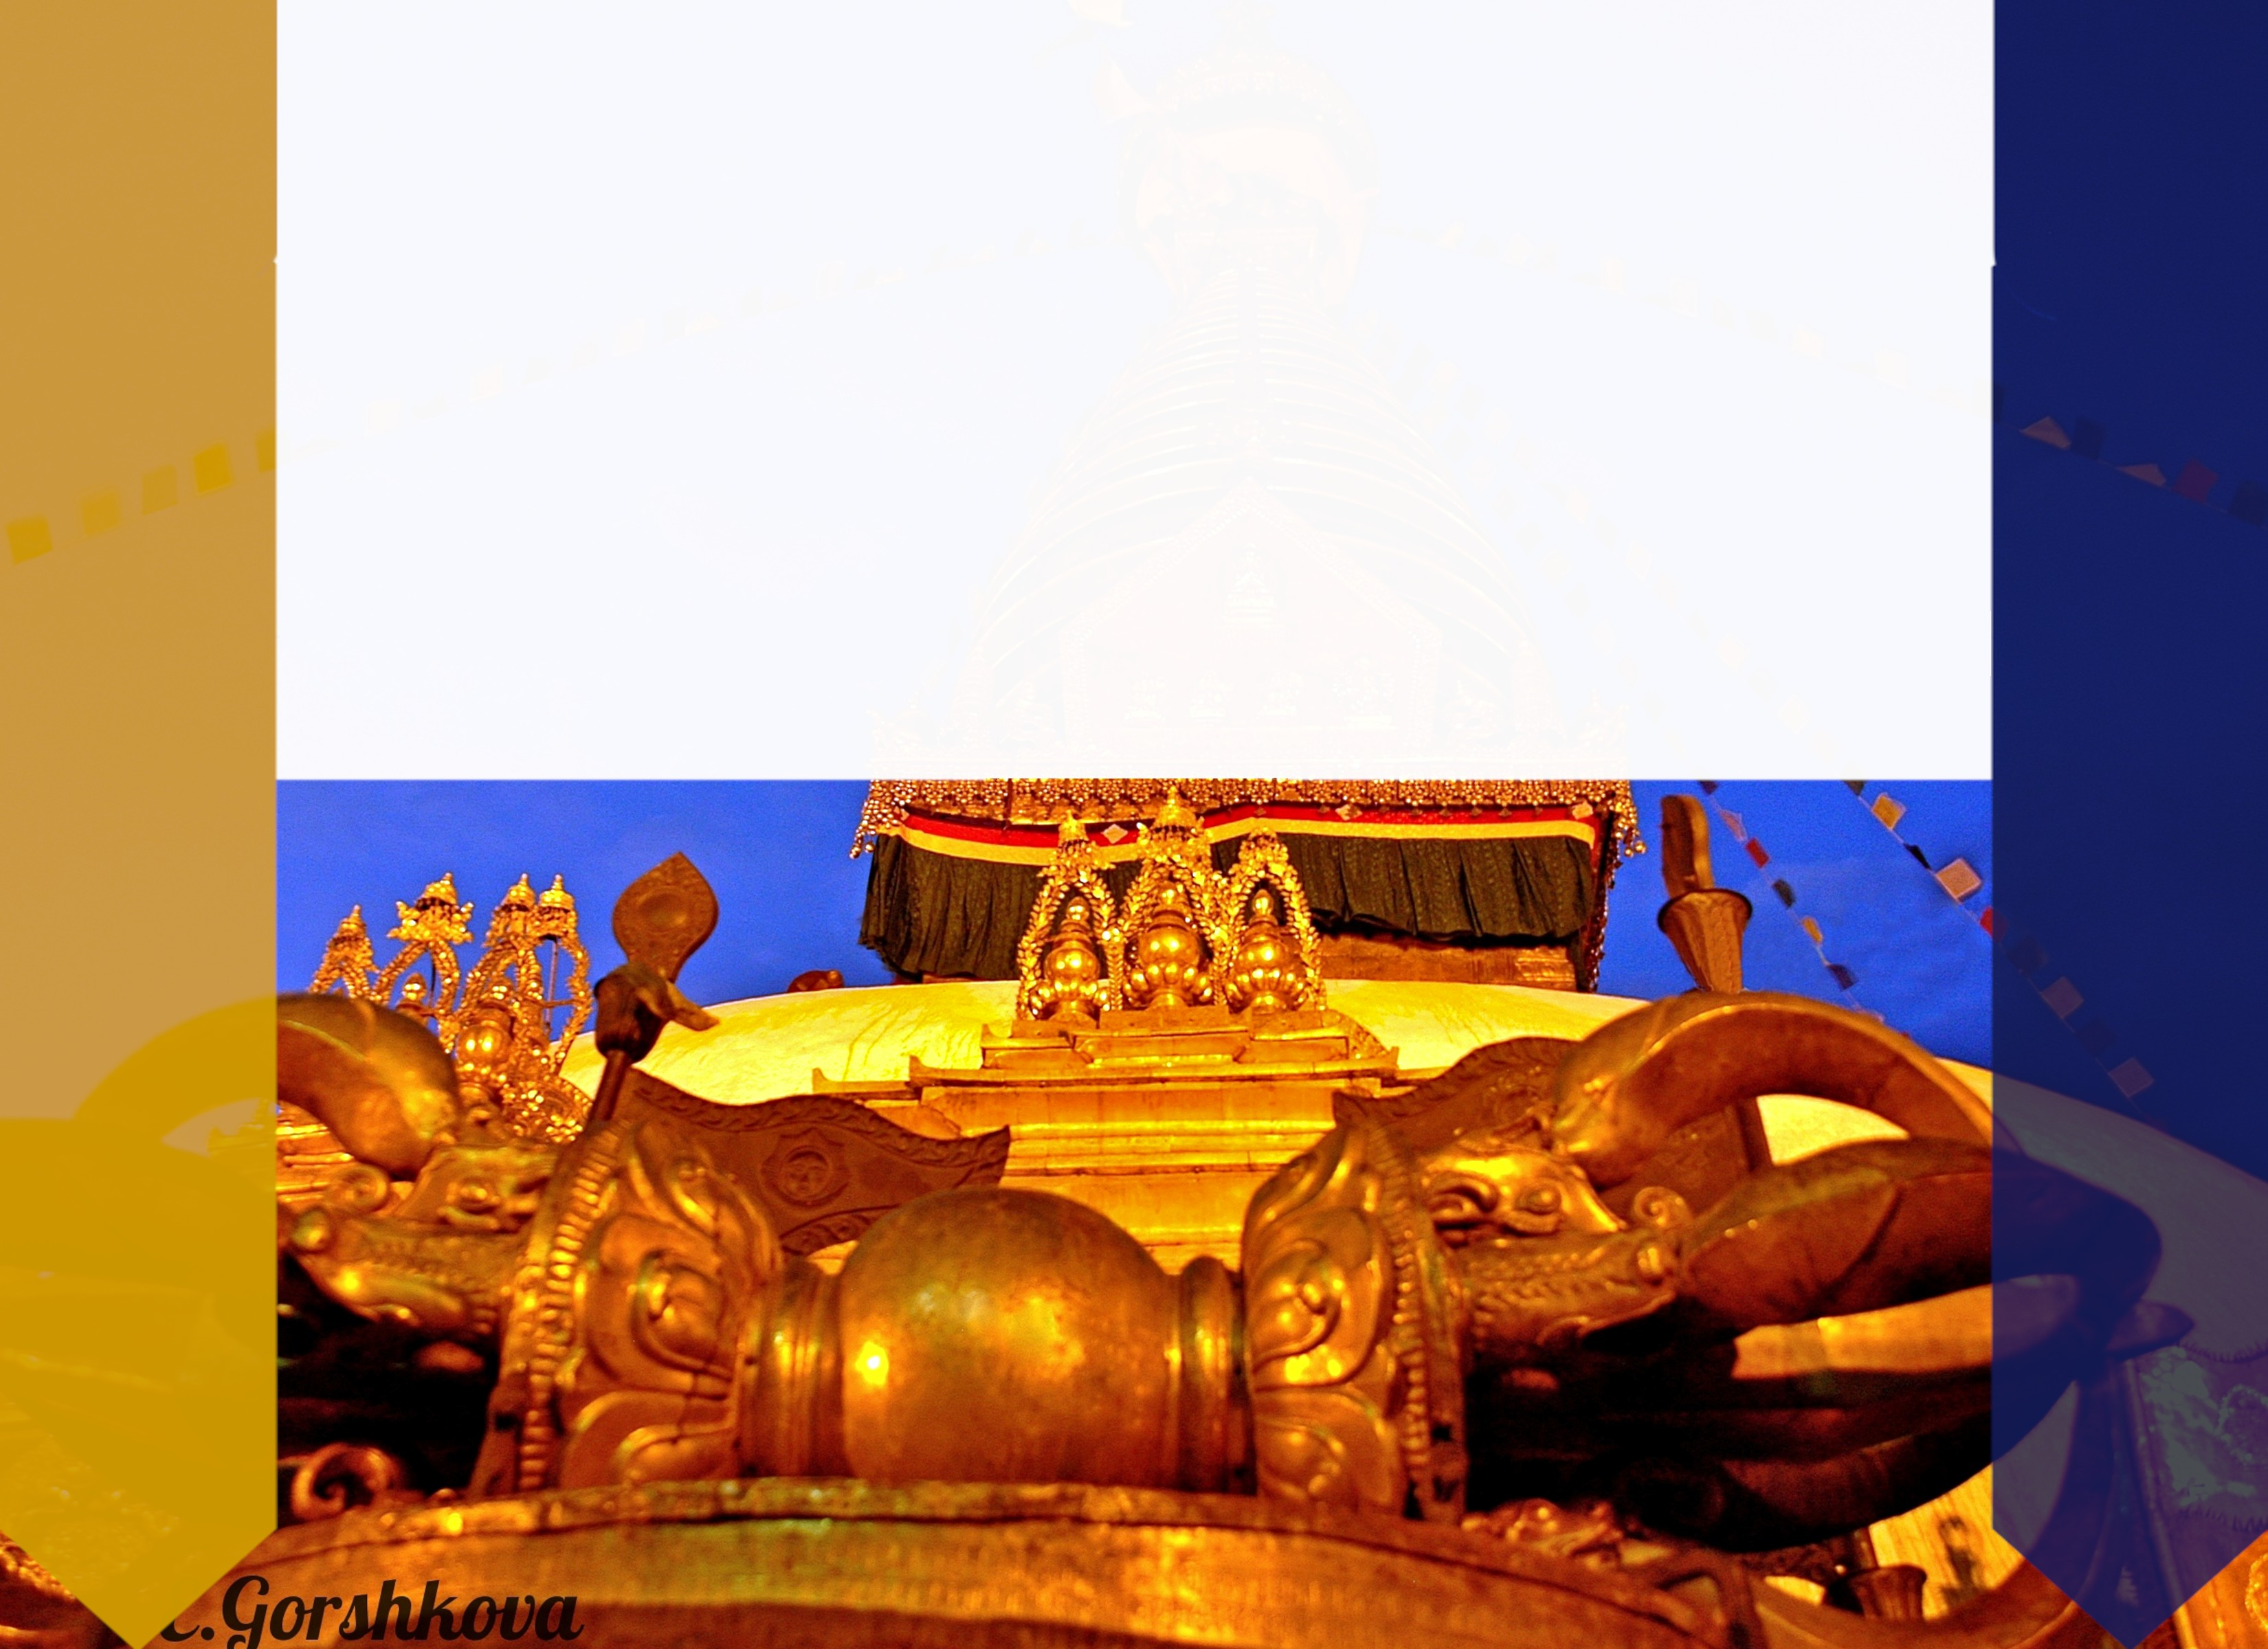
\includegraphics[width=\paperwidth,height=\paperheight]{trisula1-title.jpeg}}
\begin{titlepage} % Suppresses headers and footers on the title page
	\centering % Centre everything on the title page
	%\scshape % Use small caps for all text on the title page

	%------------------------------------------------
	%	Title
	%------------------------------------------------

	\rule{\textwidth}{1.6pt}\vspace*{-\baselineskip}\vspace*{2pt} % Thick horizontal rule
	\rule{\textwidth}{0.4pt} % Thin horizontal rule
	
	\vspace{1\baselineskip} % Whitespace above the title
	
	{\scshape\Huge The Trisula Symbol}
	
	\vspace{1\baselineskip} % Whitespace above the title

	\rule{\textwidth}{0.4pt}\vspace*{-\baselineskip}\vspace{3.2pt} % Thin horizontal rule
	\rule{\textwidth}{1.6pt} % Thick horizontal rule
	
	\vspace{1\baselineskip} % Whitespace after the title block
	
	%------------------------------------------------
	%	Subtitle
	%------------------------------------------------
	
        {\scshape By \Large William Simpson, \small ri, mras}
 
        \vspace{1.0\baselineskip}
		
        {\scshape \scriptsize Article from \\\emph{The Journal of the Royal Asiatic Society of Great Britain and Ireland}} % Subtitle or further description

	%------------------------------------------------
	%	Editor(s)
	%------------------------------------------------
        \vspace*{\fill}    

	\vspace{1\baselineskip}

        {\footnotesize\scshape London --- 1890}
	
	{\footnotesize\scshape{W. H. Allen and Co., 13, Waterloo Place, Pall Mall}}
	
	\vspace{0.25\baselineskip} % Whitespace after the title block

        {\scshape\small Internet Archive Online Edition}% Publication year}
    
	{\scshape\footnotesize Attribution NonCommercial ShareAlike 4.0 International } % Publisher
\end{titlepage}
\setlength{\parskip}{1mm plus1mm minus1mm}
\clearpage
\AddToShipoutPictureBG{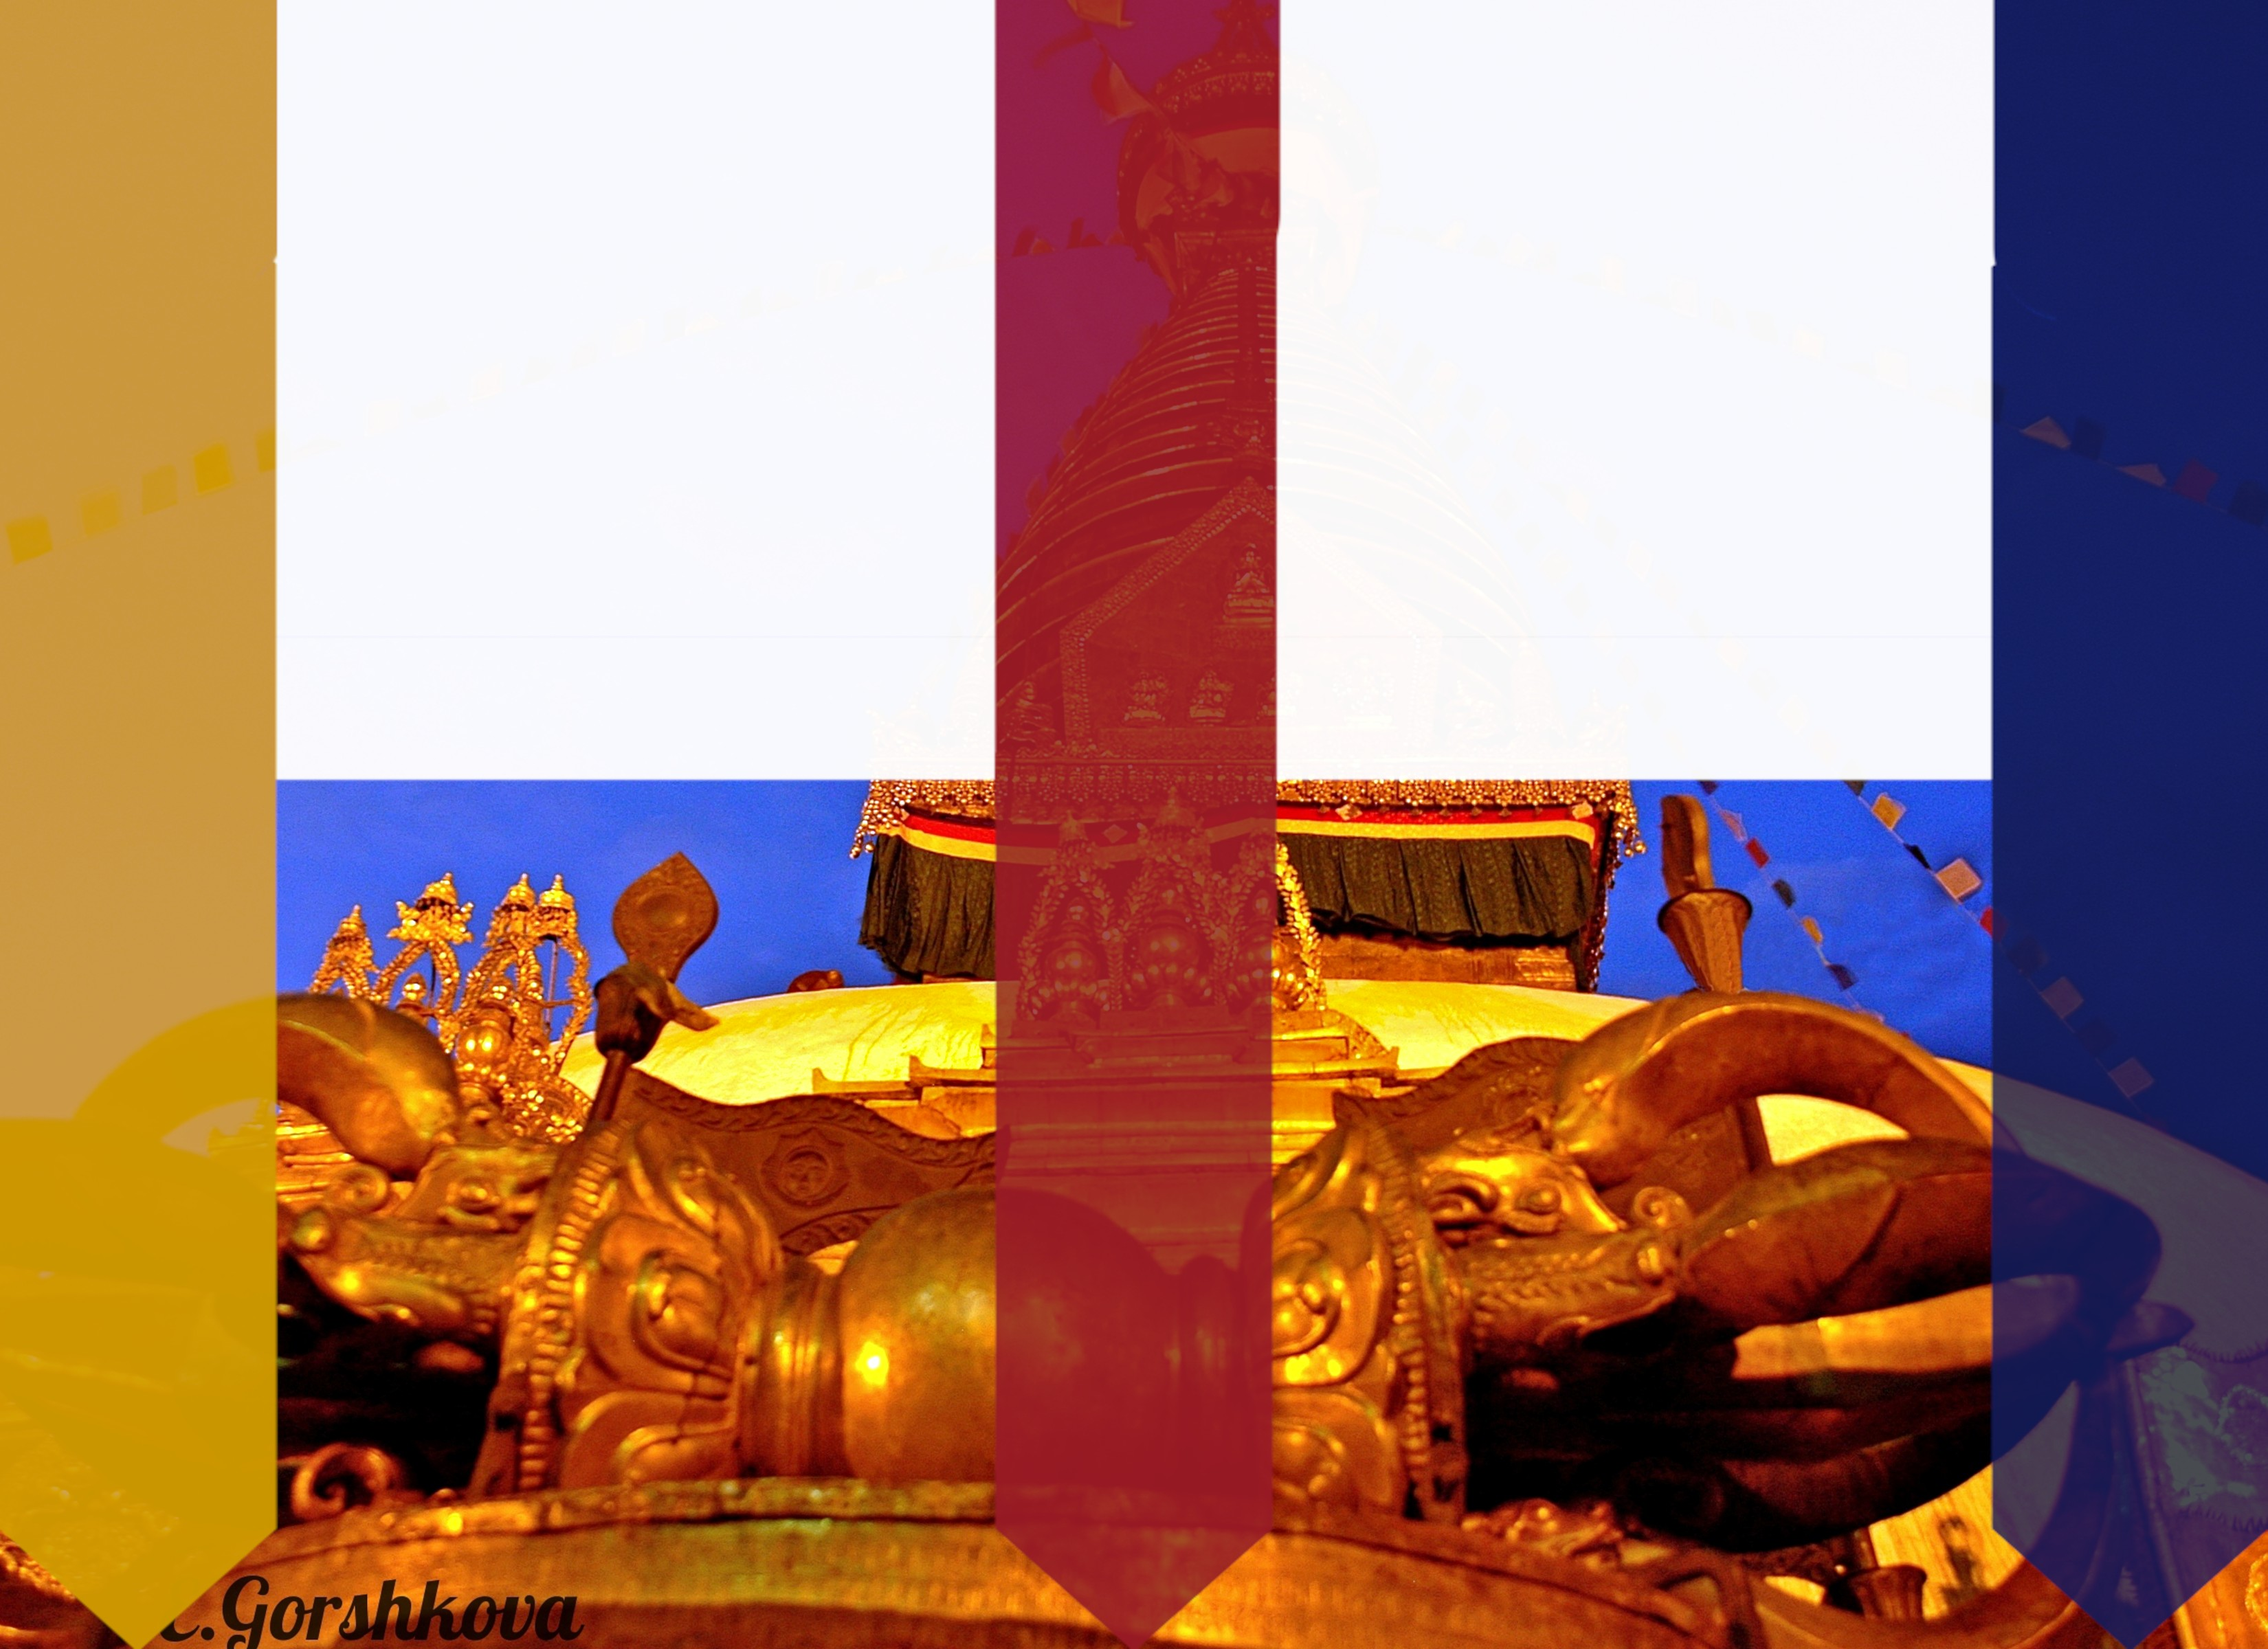
\includegraphics[width=\paperwidth,height=\paperheight]{trisula1.jpeg}}
\paragraph{}
It is only lately that the Trisula, or Trident, has attracted attention as a symbol. It so chances that for many years back I have collected matter connected with this subject, and have often wished to put it in form for publication, but want of time has always stood in the way of realizing this desire. Lately contributions dealing with the Trisula have appeared in the \emph{Journal of the Royal Asiatic Society} from Mr. Sewell and Mr. Pincott,\footnote{J. R. A. S. Vol. 18. p. 364, Vol. 19. p. 238. Fergusson, Cunningham, and others have touched upon the trisula in their works. Lately Le Comte Goblet D'Alviella, Professeur d'histoire des Religions à l'Université de Bruxelles, has published a short brochure entitled \emph{Le Trisûla ou Vardhamâna des Bouddhistes}.} and I feel urged to add some additional material to what they have given. I shall not be able to reproduce everything that I have gathered up, but my endeavour will be to give what seems to be important, or may throw light on the subject. As to a theory of origin, I have one: it has long been formed in my mind, and up to the present I see no reason to reject it; or it might be expressed, that no better theory has as yet, so far as I know, been proposed.

The symbol appears to me from what I have collected to have been very widely spread, so very ancient, and assumed such a variety of forms, that its first origin has been lost, and that now only a guess can be made as to its primitive signification. I quite agree with Mr. Pincott that the trisula is not necessarily connected with the \emph{chakra} or wheel; and that to explain the two together might leave both unexplained, because they are separate symbols. As this paper may in a sense be considered a continuation of the papers by Mr. Sewell and Mr. Pincott, I need not repeat the illustrations they have given. If the number of forms I produce in this paper are accepted as variations of the trisula, it will have to be admitted that it is one of the most important symbols of the ancient world. I should be inclined to describe it as a universal symbol, for in one form or another it is found in almost all the old systems of mythology. The theory, which appears to me to be the most probable, that the trisula is a development of solar and lunar forms, as symbols of the creative power, would, I suggest, account to a certain extent for this universality. Whether this may be the correct explanation or not, I shall be able to show that a symbol of like form with the trisula had a high significance as a monogram or letter; that a similar form was a prominent feature on sceptres in the hands of gods, priests, and kings; and that, in whatever form it appears, it had a reference to the highest of the divine attributes. While admitting the value of Mr. Sewell's essay on the possible transmission of the trisula from one locality to another, it ought to be remembered that there are other symbols, as well as myths and folklore, which are involved in this consideration; and that the explanation of one point in this broad question is of little value unless it gave us some gleam of light on the whole. If we regard the Εὶ of Delphi as a trisula, we require a theory that would suggest to us why it was placed over the gate of a temple in that part of the world, and that trisulas were placed over the gates of stupas or temples in India. This similarity may have been the result of accident, but other examples of myths and folklore might be given which are equally puzzling, but whether they are all the result of chance, or that they imply a more intimate connection between ancient nations than we have yet realized, is a matter I hesitate to venture any opinion upon. The ordinary traffic between nations might account for some of the identities; but it scarcely supplies a sufficient theory as yet to satisfy us regarding all that is known.

The first suggestion of identity with the trisula which I shall bring forward is that just alluded to of the Delphic Εὶ. In an old edition of Plutarch I have, the date of which is 1718, the essay on this subject is entitled, ``\emph{Of the Word Εὶ, Engraven over the Gate of Apollo's Temple at Delphi}.'' Plutarch explains that although called Εὶ, it was only the letter Ε, the fifth letter of the alphabet.\footnote{See Pl. 1. Fig. 19. This is from a Gnostic gem, and as it is a Greek Ε it may be accepted as accurate enough.} He says there was a golden one of Livia, wife of Augustus, and there was, or had been, a brazen one of the Athenians; to this he adds, ``but the first and ancientest of all which is the wooden one.'' The word ``engraven,'' as used above, would at first suggest that the letter was cut on the gate, but when the material of which it was formed is stated, it becomes more than probable that the symbol was a trisula, in form at least, and that it was placed ``over the gate'' of the temple. If this identification is accepted, how striking it becomes when compared with the trisulas over the gateways at Sanchi and Bharhut! It has also some force even in the case of the temples of Siva at the present day, where the trident is almost invariably placed, not on the entrance, but on the sikhara or spire. That the Εὶ of Delphi was a monogram only adds to the resemblance; for Sir Alexander Cunningham and others, although they vary in their interpretation, assume that the Buddhist trisula was also a monogram\footnote{It may be worth noting that among the various meanings ascribed to the Εὶ, Plutarch seems to adopt that which ascribes to it the sense of ``Being,'' as an attribute of the Deity, as if it was intended to express on the part of the worshipper ``Thou Art,'' or ``He'' that ``Is.'' From this some writers have identified the Εὶ with the Hebrew \<yh> or IE, pronounced \emph{Jah}, a form of the word Jehovah; the root of which is ``to be,'' ``to live,'' etc. It is easy to account for the transposition of the letters, by supposing that in one case they had been written from right to left, and in the other from left to right.}; and there are other illustrations which can be produced of this symbol in that character.

It may be noticed that Plutarch's essay shows the symbol was not clearly understood in his time. Each of the persons he has introduced as discussing its meaning gives a different explanation; in this, Plutarch's essay bears a striking resemblance to the present discussion of the trisula; the writers show very divergent opinions, and as this results from the antiquity of the symbol and absence of direct information, so Plutarch's speakers were evidently in his time in a similar condition, and it would tend to show that then, as now, the symbol was so old, that its origin had been lost, and they could only speculate regarding its meaning. If we take the explanation which Plutarch gives last as the one he most favours, it would show that he had a high notion of its symbolism. According to this it expressed the idea of Being, of that which is permanent and immutable as the character of the Deity, in opposition to the constant change and variableness which is seen in nature. This rendering would give it a sense very close to that of the celebrated ``I am that I am'' of the Pentateuch, and entitle it to an exalted rank among symbols.

I have another curious coincidence to produce, which is quite as striking as that just described. The Jews were noted for wearing frontlets or phylacteries on their foreheads. A phylactery was made of leather, and contained some passages from Scripture; on the outside of it, visible to the eye, was the Hebrew letter \emph{shin} or S.\footnote{Pl. 1. Fig. 13.} In Hebrew, Samaritan, Phœnician, in the Greek, and even in Egyptian hieroglyphics, this letter is formed more or less like a trisula.\footnote{See Pl. 1.} In the Abyssinian alphabet there are two characters to represent S, and one is a trisula in form; it is named \emph{saut}, and from being used in the word ``Negus,'' it is called the royal S.\footnote{Pl. 1. Fig. 10.} The late King Johannes, when he became King of the Kings of Ethiopia, made a change in regard to this letter; he adopted the royal S in the spelling of his name. This shows at least that there was some dignity connected with this particular form. The \emph{shin} on the phylactery is said to be the first letter of the name Shaddai, giving us another instance of this form as a monogram. Some of the Jews in the East still wear these frontlets with this symbol on them, and the coincidence will be seen from a sketch I give of a man's head from Benares.\footnote{Pl. 2. Fig. 5.} His sectarial mark is a trisula form, painted on the forehead. Of course the Hindu's explanation of the form is not the same as the Jew's; but this need not astonish us, for the symbol is understood differently in each locality where it is found. The striking thing here is that you may find a man in Jerusalem, and another in Benares, each bearing a trisula-formed symbol on his forehead.

The Hindu, whose head I sketched at Benares, said he was a worshipper of ``Seeta-Ram,'' from which it may be concluded that he was a Vaishnava. The symbol in this case is made with two colours; the external strokes and lower part are white, and the central stroke is red. In 1875 I visited Trichinopoly, and the Brahmins of the great temple of Srirangam told me this symbol is called Trinam or Trinama, and when there was a dot below, as in the sketch given,\footnote{Pl. 2. Fig. 9.} it was called Tingalynam, and that when the dot was wanting, it was called Watagalynam. This slight difference indicated a difference of faith which was not explained. All the Brahmins had these marks on their foreheads, and they were also to be seen sculptured and painted on the temples. This shows at least that the symbol occupies a prominent position in the worship of Vishnu. On asking what its signification was, it turned out, after much cross-questioning, to be male and female, or Rama and Sita. The external, or white portion, being Rama, and the Brahmins said it represented his feet, and the central stroke, which is red or saffron, represents Sita. On our way from the temple we met a man and his wife; the man had the two white strokes on his brow, and the wife had the single saffron stroke. A Brahmin, who was the friend of one of our party, explained that this was in such a case the correct form.

It may be as well to notice here that beyond the similarity of form there is no evidence that these symbols have any connection with the trisula. This will also apply to others which I shall have to bring forward. All I can say is that they are very like each other in their general character, and being important symbols, they ought to be placed in a collection of data bearing on the subject. I am inclined myself to accept them as varieties of the one symbol, but it is impossible to speak with certainty about them. I may mention that the very different explanations which are given of each cannot form an objection to their identity. The symbol is evidently very ancient, and its signification, as is the case in all symbols, would naturally be liable to changes which will suggest themselves to anyone who considers the subject.

While treating with this form in connection with letters, I had better here refer to an illustration from the Muhammadans. I do not know Arabic myself, but I have noticed in inscriptions that what I suppose to be the name of Allah is often given in an ornamental form, and in some instances it appears as a trisula. I was much struck with this in one of the tombs of the Caliphs at Cairo, where the Arabic letters are developed in this way on the top of the arched Mihrab.\footnote{Pl. 2. Fig. 8. To prevent misconception here, I may state that this illustration is not given under the notion that the Muhammadans had any idea of a trisula, hut merely to show how a sacred form may be repeated and continued by people who had no knowledge of the symbol they were using.}

There is one form in which the trisula appears, and here, in a number of cases at least, there need be no doubt about the particular symbol we are dealing with --- and that is as a sceptre. In almost every temple of Siva the trisula is to be found: it varies slightly in shape: I give sketches of it as it appears on the Golden Temple at Benares, and in an old temple near to the Golden one.\footnote{Pl. 5. Figs. 7, 8, 9.} In addition to this, Siva is, in sculpture and in pictures, generally represented with a sceptre in his hand, which is surmounted with a trisula. His sacti is often represented holding the same sceptre.

The Lamas of Tibet have a small sceptre, called a Dorjé, made of brass; it is about six inches long; it has a trident at each end. I give a drawing of one.\footnote{Pl. 3. Fig. 4. This one is exceptional, in having only the one trident at each end, but on this account it is better adapted to show the character of this ritualistic instrument.} Generally they are formed of two or four tridents, arranged in the manner to which a botanist would give the word ``whorl''; in this form the tridents at each end have the appearance of a crown. The space between the tridents, or cluster of tridents, as the case may be, at each end, is just large enough for the hand to grasp this double sceptre, for the Lamas simply held it in their hands at particular parts of the service.

The following is from Cunningham's \emph{Ladak}: ``The sceptre, \emph{dorjé}, is the Vajra of the Indians. This holy instrument is said to have flown away from India, and to have alighted at Sera, in Tibet. That it was looked upon in India, from a very early time, as an object of reverence, or as an emblem of power, is proved by its being placed in the right hand of a raja in the Sanchi bas-reliefs, which date as high as the beginning of the Christian era. It is also sculptured on the rocks at Udegiri, where it is represented in one of the hands of Durga, who is slaying Bhainsâsur. This sculpture is as old as the seventh or eighth century. In Tibetan it is called \emph{Sera-pun-dze}, and the annual festival which has been established in its honour is one of the principal religious ceremonies. The Lamas carry the sceptre in procession from Sera to Potála, where they present it to the Dalai Lama, who makes a salutation to it. They next take it to the Chinese officials, and then to the Khálons or ministers, all of whom make suitable presents of money; after which it is carried back to Sera with solemnity.''\footnote{pp. 373-4.}

There is at Buddha Gaya a stone, the traditional seat on which Buddha attained Buddhahood; of course its date is much later. It is called the \emph{Vajrásana}, or the ``thunderbolt seat''; one of the ornamental belts upon it is formed of \emph{Vajras}. The \emph{Vajra} was the thunderbolt of Indra, and this forms another attribute of the symbol, which leads again to a striking coincidence to be pointed out shortly. It may be noticed that the thunderbolt of Indra is at times described as a quoit or discus; this was also the weapon of Vishnu; as the discus and trident are both weapons of the gods, they may perhaps be only variant symbols of the same divine power. This point may be of some consideration as bearing on the \emph{Chakra}, for the discus of Vishnu goes by that name, and although not represented as a wheel, it is probably the same symbol.

Viswakarma, the architect or artificer of the gods, who corresponds with Hephaestos, is said to have formed the discus of Vishnu, the trisula of Siva, and the Vajra or thunderbolt of Indra. According to one account he made them from parings of Surya or the sun, which he put in a lathe and turned.\footnote{See \emph{Antiquities of Orissa}, by Rajendralala Mitra, vol. 2. p. 146.} This myth evidently implies a solar origin to all these weapons or symbols.

Hephaestos, the divine artificer of the Greek mythology, made the sceptre, and forged the thunderbolts of Zeus.\footnote{According to Callimachus, in the hymn to Delos, the trident of Poseidon was made by the Telchines; they also made the sickle of Chronus; these, with the discus of Vishnu, appear as weapons, but I think they should be also considered as symbols.} These thunderbolts are generally represented by an object not unlike a cigar, with a twist like a rope in it, and forked lightning projecting from each side. These of course are the later forms of the symbol. I give a representation of one of the older forms; it is from a coin I made a sketch of in the University of Athens.\footnote{P. 3. Fig. 8.} In the coins of Elis, which date about 400 \textsc{bce}, the thunderbolt of Zeus appears, under slight variations, as in this illustration. Here it is a very palpable trisula, and bearing at the same time a striking resemblance to the Vajra or thunderbolt of Indra, and appears as if it were intended to be held in the hand, as the Lamas hold the Dorjé.

Poseidon and his trident are so well known that no illustration is required. In this case the trisula seems to be a sceptre, but it is endowed with wonderful power; it was by its means that Poseidon produced the spring in the Acropolis at Athens, and also the wells in the neighbourhood of Lerna. This points again to some analogy between the trisula and the chakra, for in India there are sacred tanks and wells which Vishnu is reputed to have made with his discus. The Manikarnaka well at Benares may be mentioned as an example. Poseidon also formed the beautiful valley of Tempe with a stroke of his trident.

According to some authors Hades had a sceptre with two prongs, but I give an illustration of what I may call the medieval Hades, who carries an undoubted trisula as his sceptre.\footnote{Pl. 4. Fig. 7. This was at one time a standard subject in valentines, but the ``old gentleman'' has entirely disappeared now from this walk in art. I bought one in 1866, to keep as a popular representation of this personage, and the illustration is copied from it.}

In Rawlinson's \emph{Five Great Monarchies}\footnote{Vol. 3. p. 434.} there is an illustration representing an emblem carried in the hand of a priest. It is a peculiar form of a trisula, and is most probably a sceptre.\footnote{Pl. 4. Figs. 4, 5.}

In the Louvre is an old sceptre, which, if I mistake not, was the sceptre of Charlemagne. On my sketch I find that I have copied the following: ``Main de justice que les Rois de la troisième race ont successivement porté dans les ceremonies de leur sacre et couronnement.''\footnote{Pl. 5. Fig. 6. This sceptre is represented in the armorial bearings of the late Emperor of the French; and may be seen in some of the coins of his reign.} The hand on the top is of ivory, and the handle is gold set with gems. The fingers of the hand are in the same position as those of a bishop when he gives the benediction. The thumb and two forefingers are held up, while the other fingers are bent. I am not entitled to affirm positively that the three upright digits in this case represent a trisula, but, as we have found that so many sceptres are trisulas, it raises a strong presumption that this is only another form of that emblem.

Whatever conclusion might be come to in this instance would of course involve the hand as it is held up in the Pontifical and Episcopal blessing, for they are exactly the same in this sceptre. I give a sketch of the hand of the late Pio Nono,\footnote{Pl. 5. Fig. 2.} in the act of blessing, and with it is a sketch of the hand as held up in the Eastern Church\footnote{Pl. 5. Fig. 1.} at the present day; this, although different from the other, still shows three fingers erect. This last form is supposed to have been practised also in the Western Church during the first three or four centuries, as it is found on sarcophagi of that period, and in early mosaics.\footnote{Previous to the time of Nikon, about the middle of the seventeenth century. the benediction in the Russian Church was given with the thumb and two first fingers held up, the same as in the Latin Church, with the slight difference that the thumb and the two fingers were made to touch. The ``Old Believers'' in Russia still maintain that this is the right form. Pl. 5. Fig. 4.} I have never chanced to come upon any explanation as to how the Church invented this form of benediction with the hand, or what explanation is given regarding it. Ihe Jewish form of benediction is performed with both hands; but in each hand the two smaller fingers are separated from the middle finger, as in the hand of Pio Nono, and the two thumbs are made to touch each other.\footnote{Pl. 4. Fig. 2.} There is sufficient resemblance here to suggest some identity. In museums will be found bronze hands --- and I think there are two in the British Museum --- with the fingers in exactly the same position as in the benediction of the Latin Church\footnote{See Pl. 5. Fig. 5.}; their date I do not know, but I think they belong to the late Roman period; some of them were found in Pompeii. These hands have attached to them small figures of various kinds, such as a head like that of Jupiter or Serapis, the scales, and other signs of the Zodiac, etc. From this we may conclude that the hand in this position was a tolerably familiar symbol at one time, and that it was not exclusively Christian. The trisula being almost a universal symbol gives some probability to the supposition that the three fingers are only another form of the same. With our present knowledge I do not feel myself entitled to affirm more in relation to it. I have shown, so far as it could be made out, that the symbolism of the trisula was connected with some high attribute of the Deity, and this may perhaps be sufficient to account for the adoption by the early church of the three fingers in the act of benediction.

While dealing with the hand, I may mention the \emph{toorah} or monogram of the Sultan. A marked feature of it is three strokes which project upwards.\footnote{Pl. 1. Fig. 20.} Its being formed of letters, and that it is a monogram, is no reason against its being another form of the trisula, which I am far from being prepared to declare that it is. I give it here only as a possible contribution to the subject. When in Constantinople some years ago, I discovered that the \emph{toorah} was originally a \emph{hand}, and that it had been developed from that into its present form. I have been unable to find any of the early intermediate forms, so it is impossible on this account to say much about it. I was told that in early times the Sultan, when he had to ratify a treaty, a sheep was killed, he put his hand into the blood, and then placed it on the document as his ``hand and seal.'' Malcolm, in describing the conquests of Timour, says that ``The officers of the conqueror's army were appointed to the charge of the different provinces and cities which had been subdued, and on their commissions, instead of a seal, an impression of a red hand was stamped; a Tartar usage, that marked the manner in which the territories had been taken, as well as that in which it was intended they should be governed.''\footnote{Malcolm's \emph{History of Persia}, vol. 1. p. 465.} Although thus only a political symbol, it should be remembered that the hand had also a religious signification. There was the all-creating hand of the Supreme Being. The principal temple at Uxmal was dedicated to the God of the Working Hand; ``The open hand of Ali, called Panjeh, from the five fingers, is one of the holiest emblems of the Shias.''\footnote{\emph{Proc. Roy. Geogr. Soc.} 1884, p. 504.} Many references to the hand could be given in addition to these, but I shall add one, of which I give a sketch,\footnote{Pl. 5. Fig. 3.} it was among the emblems carried in the Sowarie of the Jeypoor Rajah when the Prince of Wales visited Jeypoor in 1876. I believe this combination of the hand and the crescent is not uncommon in India, and it may be of some value in reference to the origin of the trisula, as I incline to the theory that it is a combination of solar and lunar symbols. That there was some connection between the hand and these symbols we have the evidence of Suti monuments, where there is always represented a hand, and on each side of it the sun and moon.\footnote{``Thus we see that in the Veda-Savatar, one of the names of the sun is `Golden-Handed.' Certain it is that the early theological treatises of the Brahmins tell of the sun as having cut his hand at a sacrifice, and of the priests having replaced it by an artificial \emph{hand} made of \emph{gold}. Nay, in later times, the sun under the name of Savatar, became himself a priest; and a legend is told how, at a sacrifice, he cut off his hand, and how the other priests made a \emph{golden hand} for him.'' --- Max Müller, \emph{Science of Languages}, p. 378.}

It is not uncommon for sceptres of the west to be surmounted by a fleur-de-lis. This brings forward the question as to what the fleur-de-lis is. To this there have been a great number of explanations. The iris and lily flowers, a lance-head, bees, and frogs, have been given as the origin; these suggestions show as much variety in theory as we have in the efforts to explain the trisula. The first thing to be done in an attempt to understand a thing of this kind is to find out what we are really dealing with. The fleur-de-lis of the present day shows the members forming it continued through the cross-bar, and under the influence of the French ornamental art of last century, the whole became highly floreated. This has entirely changed the appearance of the emblem. The fleur-de-lis in this form dates only from about two centuries back; previous to that the three members of which it is formed terminated at the cross-bar, and there was only a small trefoil or handle below. In its early form it was simply a trisula. I give sketches of the modern form, and these can be compared with the older, of which I give one or two.\footnote{Pl. 3. Fig. 9, and Pl. 2. Figs. 2, 3, 7. Fig. 2 is the modern form.} The small one which forms the ground on the clasp of St. Louis is perhaps the nearest to the general appearance of the earlier period. I cannot pretend to be an authority in heraldry, but I understand that although badges and distinguishing devices are old enough, that science which is known as heraldry in our own day appeared in Europe about the time or shortly after the Crusades, and there is the probability that many of the emblems were then brought from the East, and among them the fleur-de-lis.\footnote{I have a French work, published in Paris, \emph{Recherches sur l'Origine du Blason, et en particulier sur la Fleur de Lis}, par M. Adelbert de Beaumont, which I would refer to; what I have given above, as to the period when the fleur de lis appeared in Europe, is the theory of this writer. I may mention that the fleur de lis appears in the Bayeux tapestry, and if that work of art was made immediately after the Conquest, it would throw a doubt on de Beaumont's ideas, or at least on the particular form in which he puts them. It may be also remarked that this writer does not show he has a large knowledge of the trisula, or trident, in the East. He states that ``le roi Clovis reçut d'Anastase, empereur d'Orient, le sceptre fleurdelise.'' That would be about the end of the fifth or beginning of the sixth century. This would make sceptres with the fleur-de-lis on them possible in Europe during five centuries before the Crusades; but it would still indicate an eastern origin for the emblem, a very important point in connection with this subject.}

I give what I understand to be a crown from one of the Assyrian figures in the Louvre.\footnote{Pl. 4. Fig. 3.} Bononi gives a drawing of a similar crown in \emph{Nineveh and its Palaces},\footnote{P. 434.} and in that work is a representation of Dagon\footnote{P. 168. See also Layard's \emph{Nineveh and its Remains}, vol. 2. p. 463, where it is stated that this is on a bas-relief from Khorsabad. Layard, in \emph{Discoveries in Nineveh and Babylon}, p. 343, gives another representation of this Fish-god from a gem in the British Museum which has the same crown. I have seen this often referred to as the fleur-de-lis, but it is possibly nothing more than an ornament.} with the same crown. Each of these crowns is surmounted with an ornament which is described as ``a fleur-de-lis,'' but it might be called a trisula. The same symbol appears in the British crown as a fleur-de-lis. It would be rash in the present state of our knowledge to affirm that these are all the same symbol, and that they are connected with the trisula; all that can be said is, that if the fleur-de-lis came from the East, it is just possible that it is a continuation of the important symbol we have here under consideration. It has been shown in this paper that the trisula was a divine sceptre in the hands of gods, and we may presume that it was an emblem of their supreme power; it has also been shown that priests have used the same symbol in worship; and we may here again suppose that it represented the divine attribute. In most religions priests claimed to be the Vicars of the Deity, and the Divine Right of Kings was based upon the same assumption. Having these pretensions, priests and kings would naturally use the recognized symbol as the diploma of their authority, and as evidence of the power they wielded. If the symbol was right and fitting for a sceptre, it would be right and fitting to adorn a crown.

In India the trisula became an ornament, and as a jewel was worn at an early period. On the Stupa of Bharhut there is a belt of ornament, in which the jewellery of the time is introduced as a prominent feature; there are bracelets, necklaces, bangles, etc., and among these ornaments the trisula is repeatedly given.\footnote{\emph{The Stupa of Bharhut}, by Alexander Cunningham; see Plates 43., 44., 47., 48., 49.} They are represented in pairs, but one is figured as an earring.\footnote{Pl. 3. Fig. 5.} Although worn as personal ornaments, we may suppose that they were most likely looked upon as charms, because almost all important symbols had this character ascribed to them. In the West the fleur-de-lis has long fluctuated between symbolism and ornament; and, as in many other cases, it is often difficult to say which character should be ascribed to it. In the royal crown it seems to be only a badge or mark of distinction. In the Louvre I one day noticed among the old jewellery, which was common at an early date to both Greeks and Romans, a number of objects in which the trisula form is very marked. I give illustrations of a couple of these,\footnote{Pl. 3. Figs. 6, 7.} but of course I can say nothing about the intentions of the artists who fabricated these ornaments. I have designed ornaments myself, and I am aware of the tendency there is in art of this kind to produce forms similar to the fleur-de-lis or the trisula. In architecture, particularly in Gothic, terminal ornaments are very apt to assume this character. De Beaumont's book on the fleur-de-lis, which has been already referred to, is full of these forms, most of them being, I think, only ornaments, and it rather detracts from the character of the work as an authority to find these figuring as a fleur-de-lis.

The illustrations given in this paper are sufficient to show that the trisula was a sceptre in the hands of more than one deity. As it represented in some way the divine power, it became a sceptre in the hands of priests, and was used in rites and ceremonies. If the fleur-de-lis be accepted as a form of the trisula --- but that I confess is theoretical --- this symbol appears on the sceptres of kings, representing their earthly power, but that is a natural result of the theocratical ideas which were connected with monarchy in the past; if the trisula was a symbol of divine power, the priest or king claimed to represent that power in this lower sphere. As a monogram, a very high significance was ascribed to it; as a symbol, it occupied a prominent position in temples, and men wore it on their persons as an outward mark of their faith. In every case it occupied a very sacred position, so much so that I have for a long time considered it to be about the most important of all the symbols that have come down to us. It can be traced back to a remote antiquity. I doubt if any other symbol was as widely accepted as this one was in the past; it is found over nearly the whole of the ancient world, where it figures in the Greek, Assyrian, Buddhist and Brahminical systems.

As to its origin, I incline to the theory that the trisula or trident grew out of the combination of the solar and lunar symbols. I think this is the most likely explanation, as it would account for its sacred character, as well as for its extension through so many systems. As these two symbols represented the dual creative, or re-creative power of the universe --- the power which continues all life, both animal and vegetable --- their conjunction became a fit emblem of the divine energy that preserves and rules. It expressed the power that produced cosmos out of chaos. If it symbolized the great mystery of life, either in its origin or in its continuation, it would equally symbolize the mystery of life in the future. All races have manifested a faith or hope in a life beyond death, and that death was only a re-birth into another world; and it was natural to look upon the power that first produced life and continues it as the power that would still farther preserve that life beyond the grave. If this far-reaching symbolism belonged to the trisula, it would explain the sacred character it possessed; and it would enable us to understand why it was a sceptre in the hands of gods, because it represented their highest attribute.

The development of the two symbols into the particular form of the trisula was a process which presents but little difficulty. The lunar symbol was the crescent. The full moon is a very beautiful object in the sky, but the crescent form was that which distinguished it from the round disc of the solar orb, and for this reason we may suppose it was adopted. Now the crescent is almost a universal symbol: it is found connected with nearly all the old mythologies. A collection of illustrations would be the best method of showing this symbol and its relation to the ancient systems, but that is out of the question here. It was the symbol of a large number of the principal female divinities. The great Diana of the Ephesians was not the moon, she was, as her statues show, the great mother --- the prolific Mother Earth; and the crescent was the symbol of this. All things were said to have been produced by Mother Night, or out of darkness; this was only another form of the symbolism, and it may suggest one reason why the lunar orb became connected with the power. According to this theory the central portion of the trident is supposed to have resulted from placing the solar emblem within the crescent, either as the sun itself, or as a symbol of the sun; and it thus became equivalent to the old Androgynous notion of the deity, of which traces are to be found in India, Egypt, Greece, and other parts of the world.\footnote{The Androgynous form of the deity was simply a personification of the creative power. As Ardhanari [Ardhanārīśvara] in India, it was the combined figures of Siva and Parvati. Hermaphroditus was, as the name implies, Hermes and Aphrodite. Dionysus was also represented with the twofold nature. In Egypt the Nile was represented by a figure which is distinctly male and female. Genesis 1. 27 may also be referred to. The legend of the Amazons has long been a subject of speculation; my suggestion is that they had an Androgynous type for their deity, and this, from some cause or another, came to be associated with the people of the race, and the one was confused with the other. The Ardhanari of India is perhaps a survival of the Amazonian deity, for it wants the right breast, because that side represents Siva; the left is Parvati, and has the female form of the breast.}

I shall now give some illustrations of the combination of the crescent with the sun, or the male power. The first is a rough copy of Osiris from the Serapeum at Sakkarah.\footnote{Pl. 4. Fig. 6.} The head of the figure is here surmounted by the crescent, in which is the sun.\footnote{``The orb of the sun imitated in gold is placed between the horns.'' --- \emph{Herodotus}, 2. 132.} The next is a head of Isis, in which the horns of the cow seem to represent the crescent; it is from the tomb of Psammetichus at Sakkarah.\footnote{Pl. 2. Fig. 6.} Another is the figure of Hathor,\footnote{Pl. 2. Fig. 4.} who in her attributes was closely allied to Isis; here again we have the horns inclosing the solar disc; this also was found at Sakkarah, and the originals of these are in the Museum of Bulak. The small amulets which represent the sun in Amenti become another illustration.\footnote{Pl. 1. Figs. 15, 16.} In most of these the sun is in a crescent, but in some the crescent is represented as a triangular space. These small objects, worn as charms, had a reference to the passage of the soul; each soul became Osiris, and the supposed movement of the sun in the under-world was the type. In this case it might be inferred that in these simple forms we have a symbolization of the creative power by which the individual is reborn into blessedness in the next world. That this was the meaning is, I think, fully established by the following quotation from \emph{The Book of Respirations}:
\begin{quotation}
\footnotesize
``the Book of Respirations

made by Isis for her brother Osiris,

to give life to his soul,

to give life to his body,

to rejuvenate all his members anew;

that he may reach the horizon of his father, the Sun;

that his soul may rise to heaven in the disk of the Moon.''\footnote{The Book of Respirations, \emph{Records of the Past}, vol. 4. p. 121.}
\end{quotation}
\paragraph{}
The ancient Egyptians believed in the resurrection of the body, which is indicated by the above extract, but the words also express the rebirth of the soul, thus adding a spiritual significance to the symbolization. In this case the moon becomes a kind of vehicle, but in others it appears as the place of the male power, or as a receptacle of it. In the \emph{Sîrôzahs} of the Zend books it says: ``We sacrifice unto the Moon that keeps in it the seed of the Bull.''\footnote{Yasts and Sîrôzahs, \emph{Sacred Books of the East}, vol. 23. p. 16, also at p. 8.} It is sufficient for my purpose here that the bull represents the male power, but it would be no great stretch of assumption to suppose that the bull in this instance is that of the Zodiac, which at one period was a symbol of the solar power in its recreative aspect at the vernal equinox. I give two illustrations from Rawlinson's \emph{Five Great Monarchies}, to show that the Assyrians represented the emblems of the sun god Shamas within the crescent.\footnote{Pl. 1. Figs. 17, 18.}

From the same authority I give a representation of Sin, the moon god of the Assyrians, in which we have a possible development towards the trisula form. In this the god is male, but it agrees with the other illustrations by showing the male within the female emblem.\footnote{Pl. 4. Fig. 1. I am aware that in some cases the moon was called male. This would be an important point to deal with, but its full consideration would be rather complicated to go into here. It is sufficient for my purpose that the moon was generally considered to be feminine. My own impression is that the two powers were so intimately connected as symbols, that the name of the one became the name of the other, or of both. We have many instances of this in language; the use of the word ``throne,'' when we mean the ``monarch'' who sits in it, is a good illustrative example.}

We are all familiar with the well-known legend of ``The Man in the Moon,'' who was placed there as a punishment for gathering sticks on Sunday. After what has been said about the male power in the crescent, it will strike anyone that this is either a very curious coincidence, or it is a survival of the old idea which has come down to the present day. I give an illustration of this, said to be in a church at Conway.\footnote{Pl. 1. Fig. 14.} Here again we have a development which produces a form similar to that of the trisula.

Reference may be here made again to the golden hand of the sun in the crescent, which has been already referred to. In this we have a form closely approximating to the trisula, and evidently from a development such as the theory of this paper suggests. The lingyoni of the Saiva worship might be brought forward as another illustration. In this case the female power is not represented by a crescent; but if that symbol took the place of the yoni, a perfect trisula would be the result.\footnote{The Vaisnavites, already noticed, who have the trisula painted on their foreheads, explain it as male and female, but they have somehow or another transposed the gender of the symbols.}

The Turks have adopted the crescent, embracing the sun or a star, and often in the form of a pentalpha; the crescent in this case is supposed to have been derived from the old Byzantine symbolism; and traces of this symbolism are still to be found in the Eastern Church. The Russian Church, which owes its origin to Byzantium, places a crescent under the cross,\footnote{See Pl. 3. Fig. 1.} an arrangement which is much older than what is called the ``triumph of the cross over the crescent,'' that being the usual explanation. The Abyssinian Church also places a curved form under their large processional crosses, which looks as if it were derived from the crescent.\footnote{See Pl. 3. Figs. 2, 3.}

These examples are produced merely to show that if a crescent form is adopted, and a symbol, solar or otherwise, is placed within it, how easily the trisula symbol might be evolved.

Many other illustrations might be given which would help to support the theory of the origin of the trisula I have ventured to suggest. I cannot affirm that the theory has been established into a certainty. All I can say is that the view of the case here presented is the one which seems to me to be the most probable, and that which is in the greatest conformity with the data I have produced. The illustrations given will show that the trisula had from a far back period a wide acceptance as a symbol over a large geographical space. How to account for this is a difficulty which belongs to many other matters connected with mythology and symbolism. Whether ideas in the past were carried from one nation to another by means of commerce, conquest or immigration, or had separate developments, is a problem in many cases I think we are as yet far from being in a position to solve in a satisfactory manner. Whatever may have been the origin of the trisula, if its existence in countries so widely separated could be explained, the solution would be a most valuable contribution to our knowledge of mythology.
\clearpage
\begin{figure}[H]
\centering
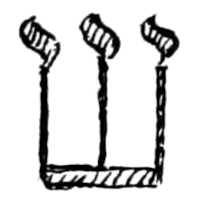
\includegraphics[width=0.25\textwidth,keepaspectratio]{figs/1-1.png}
\caption{Plate 1. --- Fig. 1: Forms of the Hebrew S, or \emph{Shin}.}
\end{figure}

\begin{figure}[H]
\centering
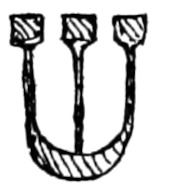
\includegraphics[width=0.25\textwidth,keepaspectratio]{figs/1-2.png}
\caption{Plate 1. --- Fig. 2: Forms of the Hebrew S, or \emph{Shin}.}
\end{figure}

\begin{figure}[H]
\centering
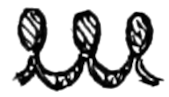
\includegraphics[width=0.25\textwidth,keepaspectratio]{figs/1-3.png}
\caption{Plate 1. --- Fig. 3: Samaritan Shin.}
\end{figure}

\begin{figure}[H]
\centering
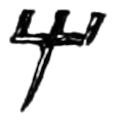
\includegraphics[width=0.25\textwidth,keepaspectratio]{figs/1-4.png}
\caption{Plate 1. --- Fig. 4: Phœnician Forms.}
\end{figure}

\begin{figure}[H]
\centering
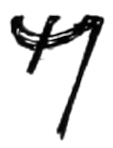
\includegraphics[width=0.25\textwidth,keepaspectratio]{figs/1-5.png}
\caption{Plate 1. --- Fig. 5: Phœnician Forms.}
\end{figure}

\begin{figure}[H]
\centering
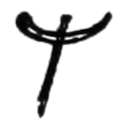
\includegraphics[width=0.25\textwidth,keepaspectratio]{figs/1-6.png}
\caption{Plate 1. --- Fig. 6: Phœnician Forms.}
\end{figure}

\begin{figure}[H]
\centering
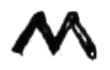
\includegraphics[width=0.25\textwidth,keepaspectratio]{figs/1-7.png}
\caption{Plate 1. --- Fig. 7: Greek.}
\end{figure}

\begin{figure}[H]
\centering
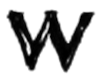
\includegraphics[width=0.25\textwidth,keepaspectratio]{figs/1-8.png}
\caption{Plate 1. --- Fig. 8: Ancient Hebrew Shins.}
\end{figure}

\begin{figure}[H]
\centering
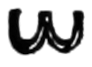
\includegraphics[width=0.25\textwidth,keepaspectratio]{figs/1-9.png}
\caption{Plate 1. --- Fig. 9: Ancient Hebrew Shins.}
\end{figure}

\begin{figure}[H]
\centering
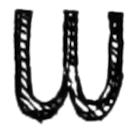
\includegraphics[width=0.25\textwidth,keepaspectratio]{figs/1-10.png}
\caption{Plate 1. --- Fig. 10: \emph{Saut}, The Royal S of the Abyssinian Alphabet.}
\end{figure}

\begin{figure}[H]
\centering
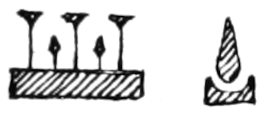
\includegraphics[width=0.25\textwidth,keepaspectratio]{figs/1-11.png}
\caption{Plate 1. --- Fig. 11: SH in Egyptian Hieroglyphics.}
\end{figure}

\begin{figure}[H]
\centering
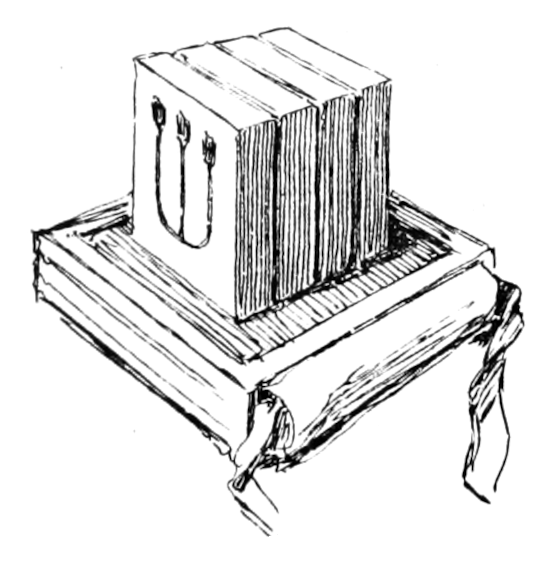
\includegraphics[width=0.25\textwidth,keepaspectratio]{figs/1-13.png}
\caption{Plate 1. --- Fig. 13: The Phylactery of the Jews.}
\end{figure}

\begin{figure}[H]
\centering
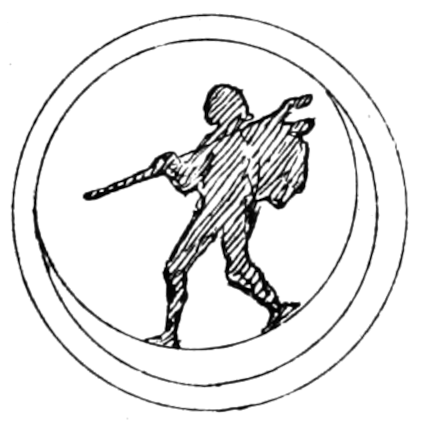
\includegraphics[width=0.25\textwidth,keepaspectratio]{figs/1-14.png}
\caption{Plate 1. --- Fig. 14: The ``Man in the Moon.''}
\end{figure}

\begin{figure}[H]
\centering
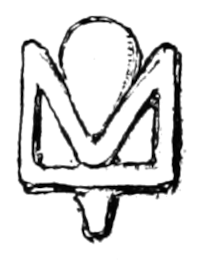
\includegraphics[width=0.25\textwidth,keepaspectratio]{figs/1-15.png}
\caption{Plate 1. --- Fig. 15: The Sun in Amenti.}
\end{figure}

\begin{figure}[H]
\centering
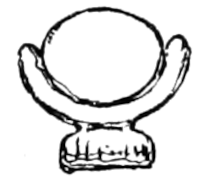
\includegraphics[width=0.25\textwidth,keepaspectratio]{figs/1-16.png}
\caption{Plate 1. --- Fig. 16: The Sun in Amenti.}
\end{figure}

\begin{figure}[H]
\centering
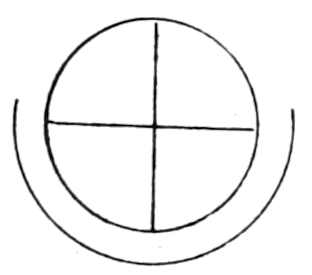
\includegraphics[width=0.25\textwidth,keepaspectratio]{figs/1-17.png}
\caption{Plate 1. --- Fig. 17: Sun God Shamas, Assyrian.}
\end{figure}

\begin{figure}[H]
\centering
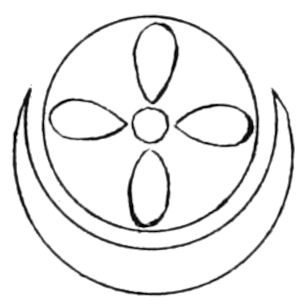
\includegraphics[width=0.25\textwidth,keepaspectratio]{figs/1-18.png}
\caption{Plate 1. --- Fig. 18: Sun God Shamas, Assyrian.}
\end{figure}

\begin{figure}[H]
\centering
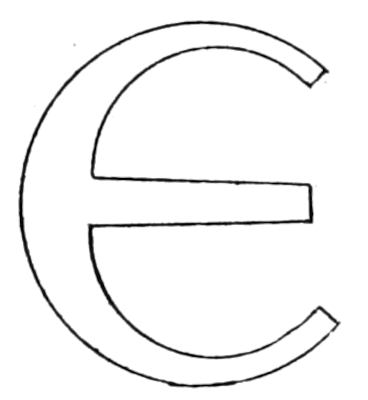
\includegraphics[width=0.25\textwidth,keepaspectratio]{figs/1-19.png}
\caption{Plate 1. --- Fig. 19: The Εὶ of Delphi.}
\end{figure}

\begin{figure}[H]
\centering
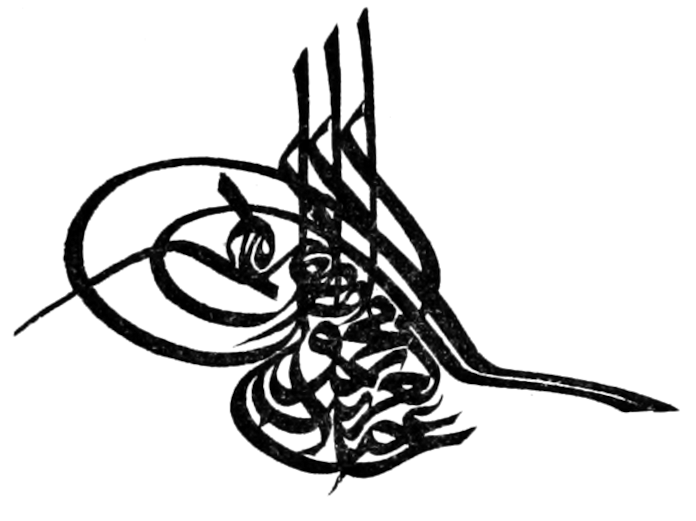
\includegraphics[width=0.35\textwidth,keepaspectratio]{figs/1-20.png}
\caption{Plate 1. --- Fig. 20: The Sultan's Toorah.}
\end{figure}

\begin{figure}[H]
\centering
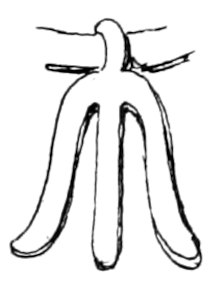
\includegraphics[width=0.25\textwidth,keepaspectratio]{figs/2-1.png}
\caption{Plate 2. --- Fig. 1: Symbol from Royal Collar, Nimroud.}
\end{figure}

\begin{figure}[H]
\centering
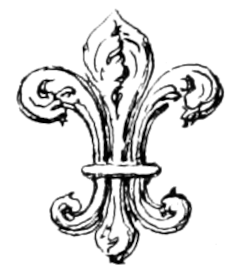
\includegraphics[width=0.25\textwidth,keepaspectratio]{figs/2-2.png}
\caption{Plate 2. --- Fig. 2: Late Fleur-de-lis.}
\end{figure}

\begin{figure}[H]
\centering
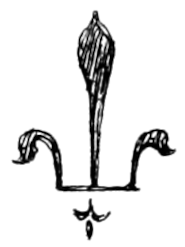
\includegraphics[width=0.25\textwidth,keepaspectratio]{figs/2-3.png}
\caption{Plate 2. --- Fig. 3: Older form of Fleur-de-lis.}
\end{figure}

\begin{figure}[H]
\centering
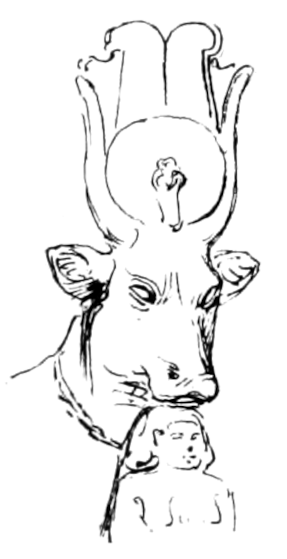
\includegraphics[width=0.15\textwidth,keepaspectratio]{figs/2-4.png}
\caption{Plate 2. --- Fig. 4: Hathor with Solar Disc in Horns.}
\end{figure}

\begin{figure}[H]
\centering
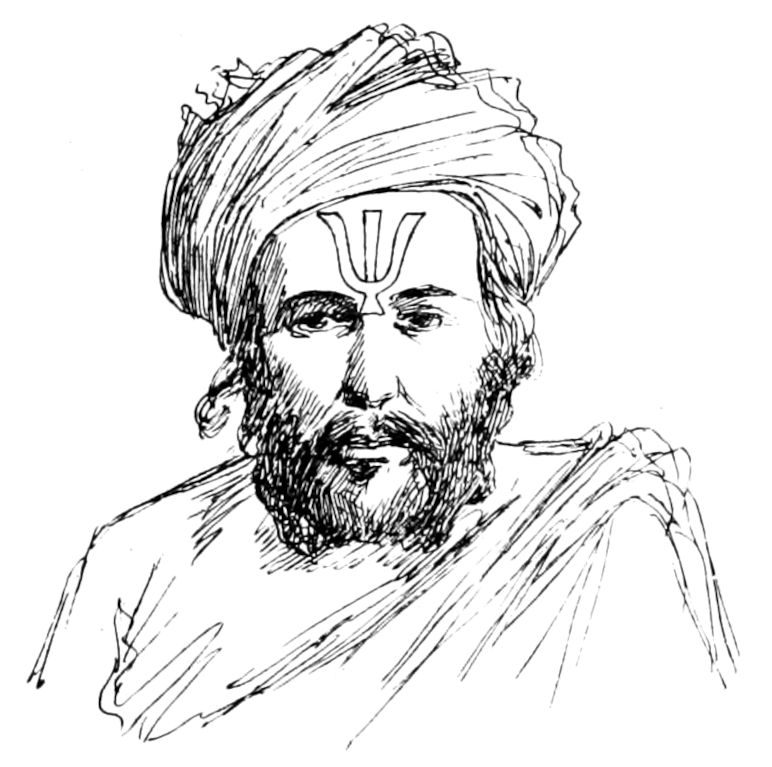
\includegraphics[width=0.3\textwidth,keepaspectratio]{figs/2-5.png}
\caption{Plate 2. --- Fig. 5: Head of a Vishnaiva, Benares.}
\end{figure}

\begin{figure}[H]
\centering
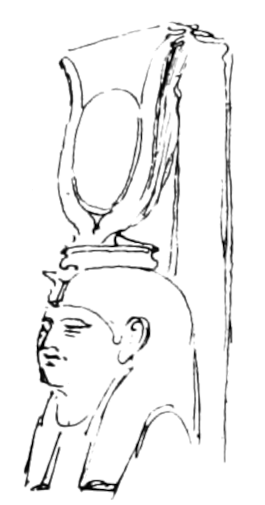
\includegraphics[width=0.15\textwidth,keepaspectratio]{figs/2-6.png}
\caption{Plate 2. --- Fig. 6: Isis with Solar Disc in Horns.}
\end{figure}

\begin{figure}[H]
\centering
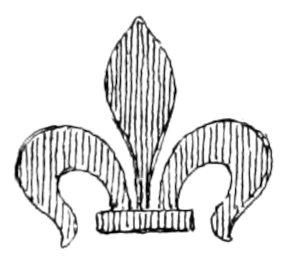
\includegraphics[width=0.25\textwidth,keepaspectratio]{figs/2-7.png}
\caption{Plate 2. --- Fig. 7: Old form of Fleur-de-lis.}
\end{figure}

\begin{figure}[H]
\centering
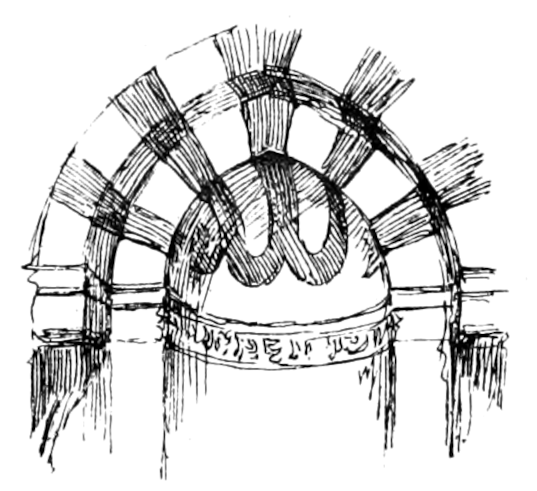
\includegraphics[width=0.25\textwidth,keepaspectratio]{figs/2-8.png}
\caption{Plate 2. --- Fig. 8: Mihrab, Tomb of the Caliphs, Cairo.}
\end{figure}

\begin{figure}[H]
\centering
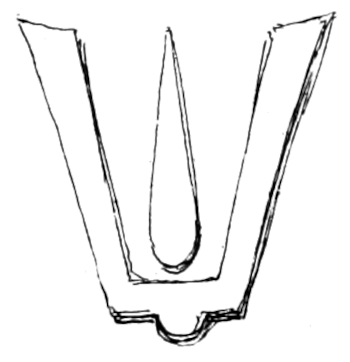
\includegraphics[width=0.25\textwidth,keepaspectratio]{figs/2-9.png}
\caption{Plate 2. --- Fig. 9: Tingalynam.}
\end{figure}

\begin{figure}[H]
\centering
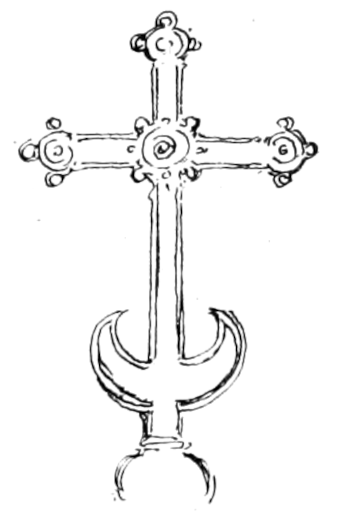
\includegraphics[width=0.2\textwidth,keepaspectratio]{figs/3-1.png}
\caption{Plate 3. --- Fig. 1: Russian Cross with Crescent.}
\end{figure}

\begin{figure}[H]
\centering
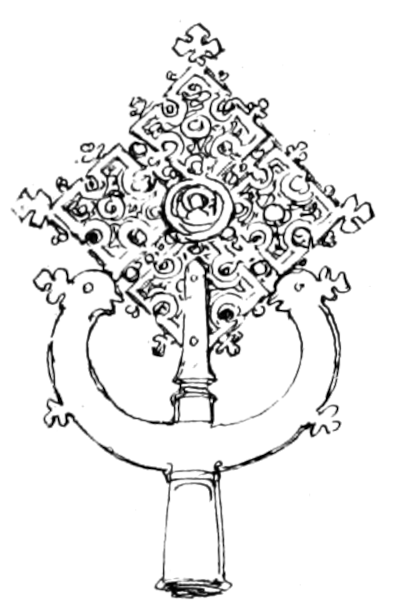
\includegraphics[width=0.2\textwidth,keepaspectratio]{figs/3-2.png}
\caption{Plate 3. --- Fig. 2: Abyssinian Crosses.}
\end{figure}

\begin{figure}[H]
\centering
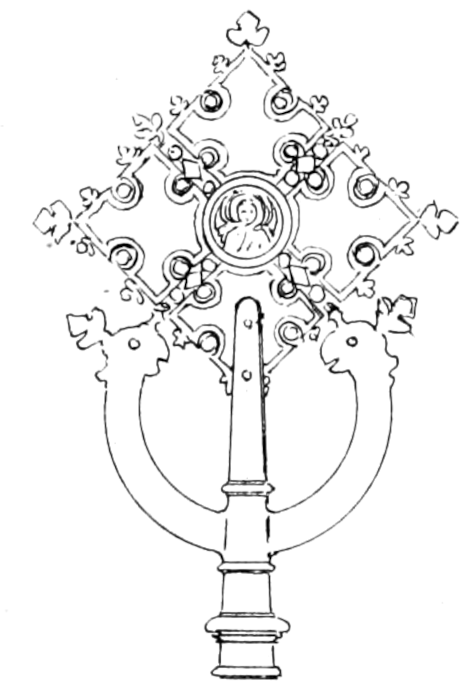
\includegraphics[width=0.2\textwidth,keepaspectratio]{figs/3-3.png}
\caption{Plate 3. --- Fig. 3: Abyssinian Crosses.}
\end{figure}

\begin{figure}[H]
\centering
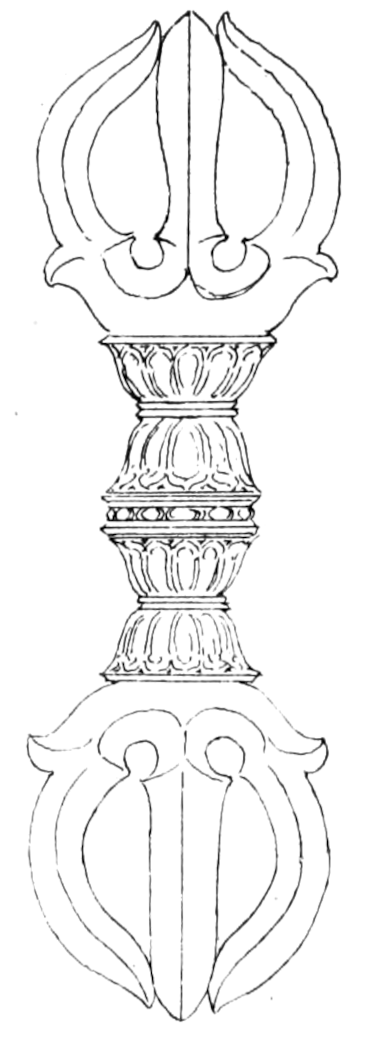
\includegraphics[width=0.13\textwidth,keepaspectratio]{figs/3-4.png}
\caption{Plate 3. --- Fig. 4: Tibetan Dorjé.}
\end{figure}

\begin{figure}[H]
\centering
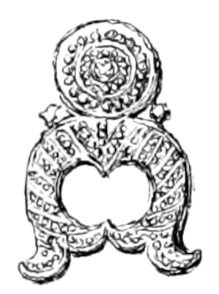
\includegraphics[width=0.2\textwidth,keepaspectratio]{figs/3-5.png}
\caption{Plate 3. --- Fig. 5: Trisula as an Ornament, Bharhut.}
\end{figure}

\begin{figure}[H]
\centering
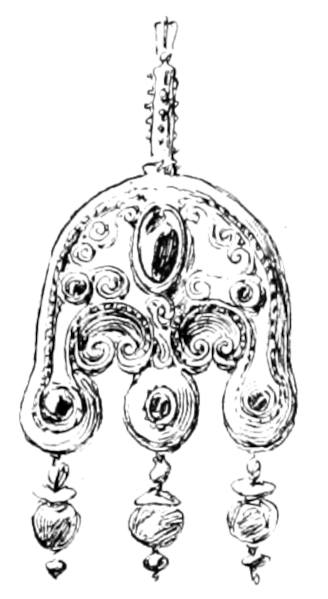
\includegraphics[width=0.15\textwidth,keepaspectratio]{figs/3-6.png}
\caption{Plate 3. --- Fig. 6: Greek Gold Ornaments, Louvre.}
\end{figure}

\begin{figure}[H]
\centering
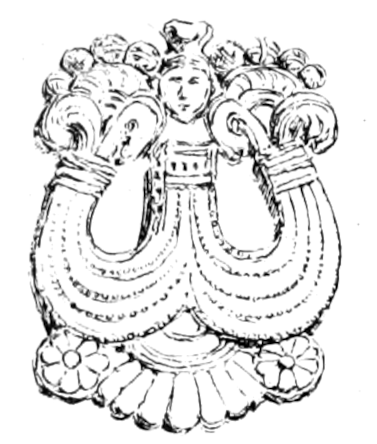
\includegraphics[width=0.25\textwidth,keepaspectratio]{figs/3-7.png}
\caption{Plate 3. --- Fig. 7: Greek Gold Ornaments, Louvre.}
\end{figure}

\begin{figure}[H]
\centering
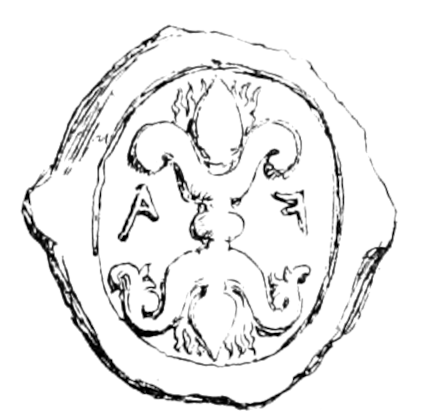
\includegraphics[width=0.25\textwidth,keepaspectratio]{figs/3-8.png}
\caption{Plate 3. --- Fig. 8: Coin of Elis, 4\textsuperscript{th} cent. \textsc{bce}.}
\end{figure}

\begin{figure}[H]
\centering
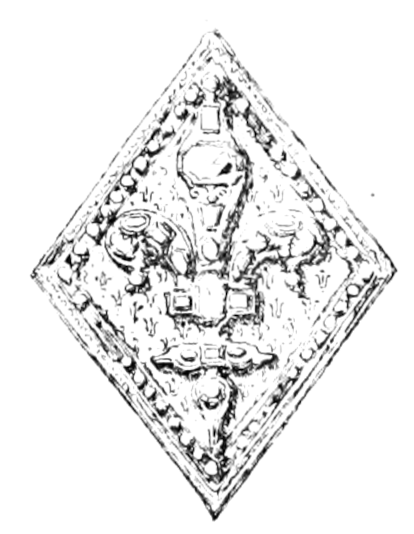
\includegraphics[width=0.25\textwidth,keepaspectratio]{figs/3-9.png}
\caption{Plate 3. --- Fig. 9: Fleur-de-lis on the Clasp of Mantle of St. Louis, 1226-1270 \textsc{ce}, Louvre.}
\end{figure}

\begin{figure}[H]
\centering
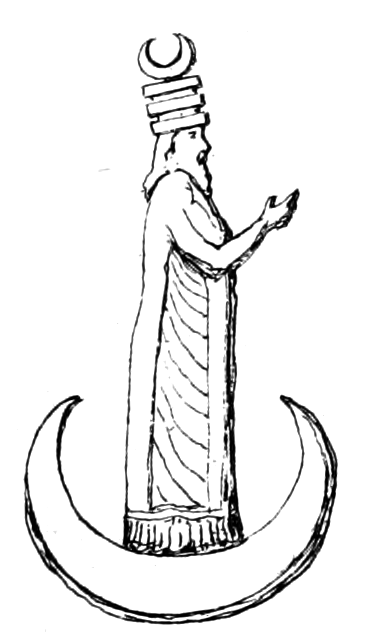
\includegraphics[width=0.2\textwidth,keepaspectratio]{figs/4-1.png}
\caption{Plate 4. --- Fig. 1: Sin or the Moon God, Assyrian.}
\end{figure}

\begin{figure}[H]
\centering
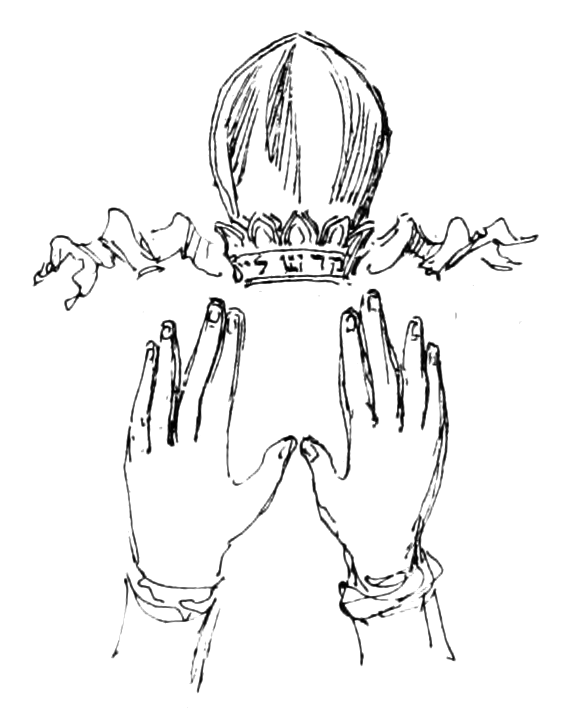
\includegraphics[width=0.25\textwidth,keepaspectratio]{figs/4-2.png}
\caption{Plate 4. --- Fig. 2: Hebrew form of Benediction.}
\end{figure}

\begin{figure}[H]
\centering
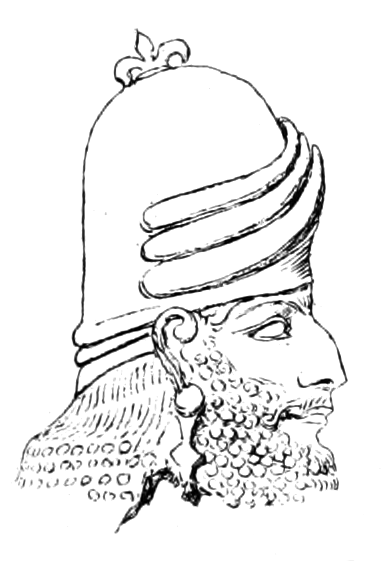
\includegraphics[width=0.2\textwidth,keepaspectratio]{figs/4-3.png}
\caption{Plate 4. --- Fig. 3: Assyrian, Louvre.}
\end{figure}

\begin{figure}[H]
\centering
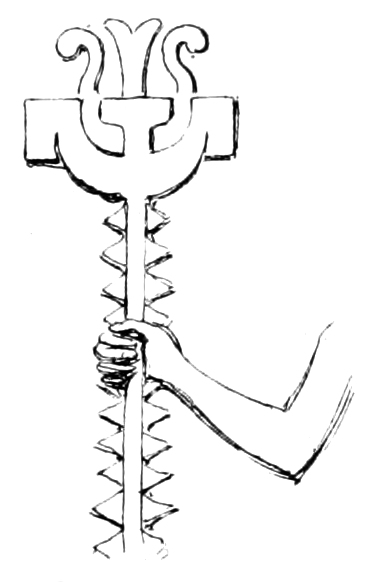
\includegraphics[width=0.2\textwidth,keepaspectratio]{figs/4-4.png}
\caption{Plate 4. --- Fig. 4: Emblem carried by Babylonian Priest.}
\end{figure}

\begin{figure}[H]
\centering
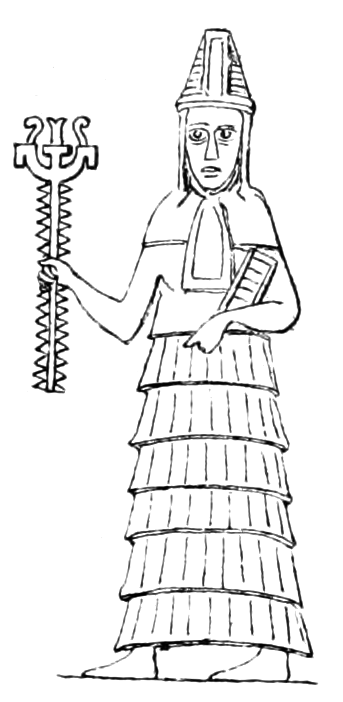
\includegraphics[width=0.15\textwidth,keepaspectratio]{figs/4-5.png}
\caption{Plate 4. --- Fig. 5: Babylonian Priest.}
\end{figure}

\begin{figure}[H]
\centering
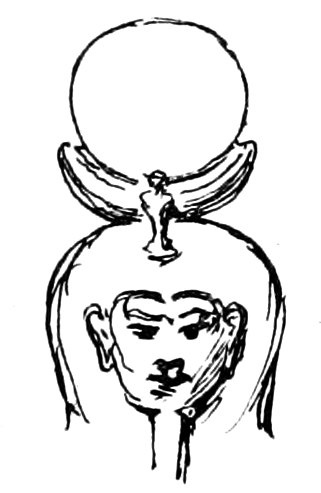
\includegraphics[width=0.15\textwidth,keepaspectratio]{figs/4-6.png}
\caption{Plate 4. --- Fig. 6: Osiris.}
\end{figure}

\begin{figure}[H]
\centering
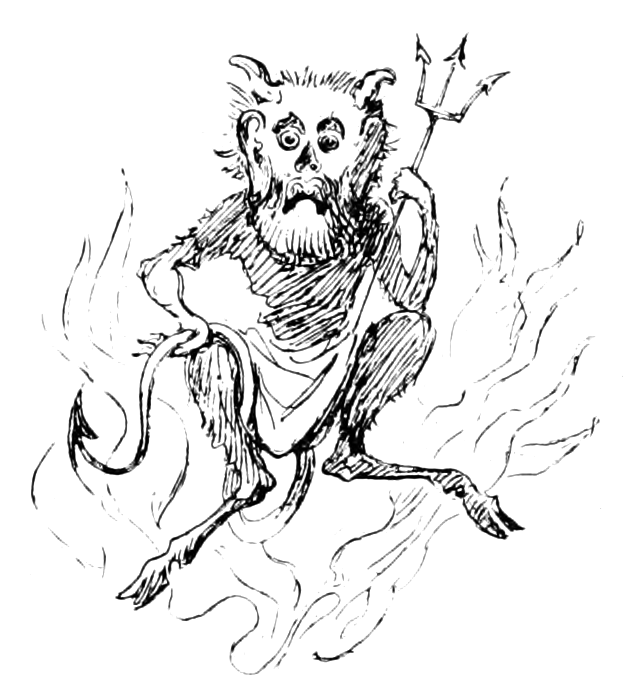
\includegraphics[width=0.25\textwidth,keepaspectratio]{figs/4-7.png}
\caption{Plate 4. --- Fig. 7: Medieval Satan.}
\end{figure}

\begin{figure}[H]
\centering
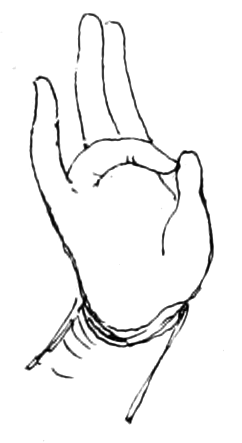
\includegraphics[width=0.15\textwidth,keepaspectratio]{figs/5-1.png}
\caption{Plate 5. --- Fig. 1: Greek form of Hand in Benediction.}
\end{figure}

\begin{figure}[H]
\centering
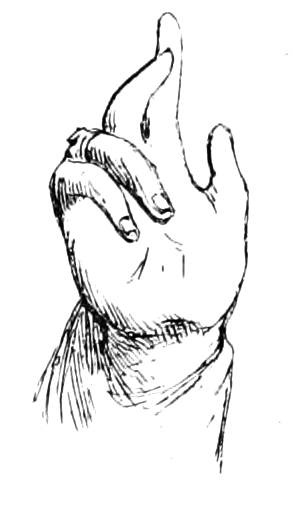
\includegraphics[width=0.2\textwidth,keepaspectratio]{figs/5-2.png}
\caption{Plate 5. --- Fig. 2: The Papal Hand.}
\end{figure}

\begin{figure}[H]
\centering
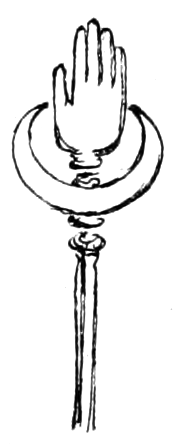
\includegraphics[width=0.15\textwidth,keepaspectratio]{figs/5-3.png}
\caption{Plate 5. --- Fig. 3: Symbol carried at Jeypoor.}
\end{figure}

\begin{figure}[H]
\centering
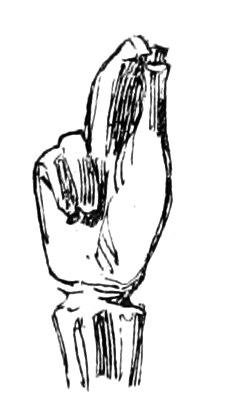
\includegraphics[width=0.15\textwidth,keepaspectratio]{figs/5-4.png}
\caption{Plate 5. --- Fig. 4: Hand in Russian Church, before time of Nikon.}
\end{figure}

\begin{figure}[H]
\centering
\includegraphics[width=0.15\textwidth,keepaspectratio]{figs/5-5.png}
\caption{Plate 5. --- Fig. 5: Old Bronze Hand.}
\end{figure}

\begin{figure}[H]
\centering
\includegraphics[width=0.1\textwidth,keepaspectratio]{figs/5-6.png}
\caption{Plate 5. --- Fig. 6: Sceptre of Charlemagne, Louvre.}
\end{figure}

\begin{figure}[H]
\centering
\includegraphics[width=0.15\textwidth,keepaspectratio]{figs/5-7.png}
\caption{Plate 5. --- Fig. 7: Trisulas of Siva.}
\end{figure}

\begin{figure}[H]
\centering
\includegraphics[width=0.15\textwidth,keepaspectratio]{figs/5-8.png}
\caption{Plate 5. --- Fig. 8: Trisulas of Siva.}
\end{figure}

\begin{figure}[H]
\centering
\includegraphics[width=0.15\textwidth,keepaspectratio]{figs/5-9.png}
\caption{Plate 5. --- Fig. 9: Trisulas of Siva.}
\end{figure}
\clearpage
\end{document}
